\documentclass[class=report, crop=false]{standalone}
\usepackage[subpreambles=true]{standalone}
\usepackage{import}
%%\usepackage{booktabs}
%\usepackage{tikz}

%\usepackage[utf8]{inputenc}
\usepackage[subpreambles=true]{standalone}
\usepackage{import}
\usepackage{pgfplots}
\pgfplotsset{compat=newest}
\usepgfplotslibrary{groupplots}
\usepgfplotslibrary{dateplot}
\usepackage{caption}
\usepackage{subcaption}
\usepackage{graphicx}
\usepackage{amsmath}
\usepackage{amssymb}
\usepackage[parfill]{parskip}
\usepackage{float}

% \usepackage{pgfplots}
% \usetikzlibrary{pgfplots.groupplots}
% \pgfplotsset{compat=1.9,height=0.3\textheight,legend cell align=left,tick scale binop=\times}
% \pgfplotsset{grid style={loosely dotted,color=darkgray!30!gray,line width=0.6pt},tick style={black,thin}}
% \pgfplotsset{every axis plot/.append style={line width=0.8pt}}
%
% \usepgfplotslibrary{external}
% % Für die Verwendung von 'external' müssen die folgenden Anpassungen in Abhängigkeit der
% % LaTeX Distribution durchgeführt werden:
%
% % fuer Texlive: pdflatex.exe -shell-escape -synctex=1 -interaction=nonstopmode %.tex
% \tikzexternalize[shell escape=-shell-escape]   % fuer TeXLive
%
% % fuer MikTeX:  pdflatex.exe -enable-write18 -synctex=1 -interaction=nonstopmode %.tex
% %\tikzexternalize[shell escape=-enable-write18] % fuer MikTex
%
%
%
% \tikzsetexternalprefix{graphics/pgfplots/} % Ordner muss ev. zuerst haendisch erstellt werden

\begin{document}

\chapter{Approach}\label{cha:approach}
\pagestyle{scrheadings}
The rise in popularity of the maker culture, which democratizes access to STEM and other tech-rich domains, has enabled large scale production of cheap plug-and-play components which can be utilized not just for hobby projects, but also for research purposes.

Our platform was designed around such products to be as low cost as reasonably possible. Our choice of parts was dictated mainly by already freely available. The missing parts were bought with a low price in mind to explore what could be possible with such design restrictions.

Wheel encoders for our platform were too costly to incorporate, this is why we used a fake wheel encoder which is the motor forward signal from the joystick. We inspect the accuracy and usefullness of this signal used in conjunction with an IMU through experiments.

\begin{SCfigure}
  \centering
    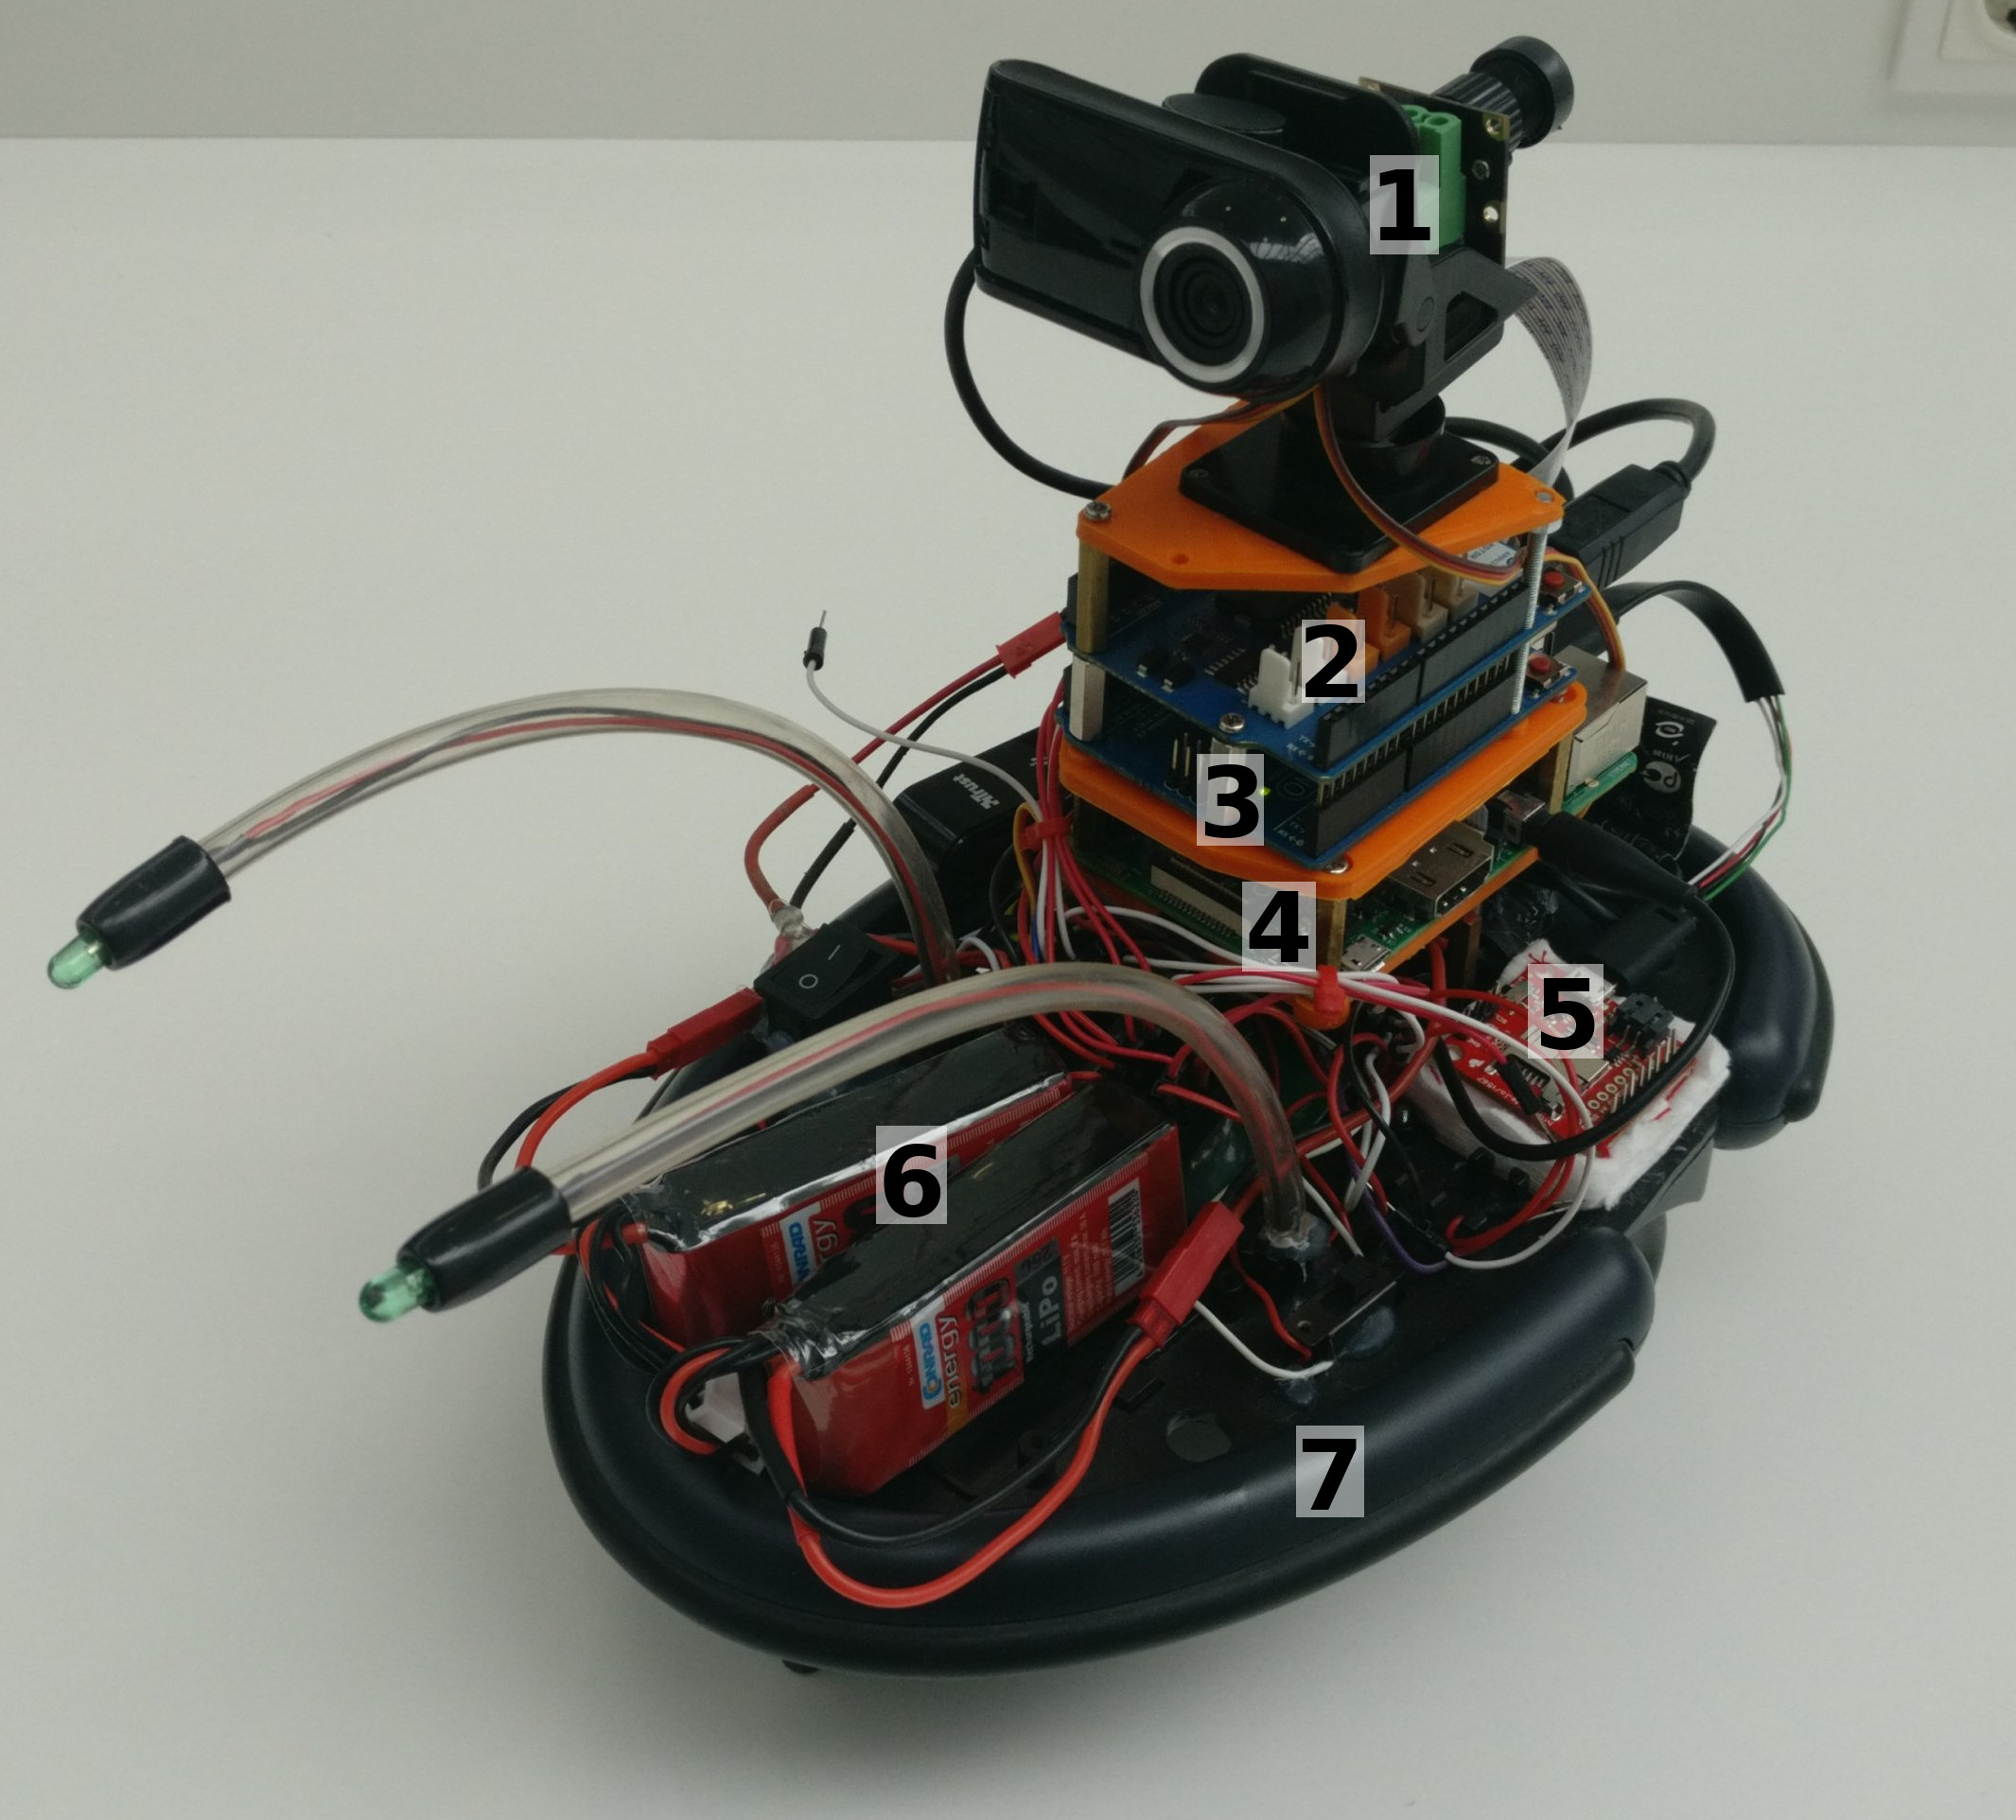
\includegraphics[width=8cm]{images/profile_numbered}
    \caption{\\Platform parts:\\1: Camera\\2: Motor Shield\\3: Arduino UNO\\
    4: Raspberry Pi 3\\5: Razor IMU\\6: LiPo Batteries\\7: Chassis}
\end{SCfigure}

\import{sections/}{hardware}

\import{sections/}{software}

\end{document}
